%!TEX root = skripsi.tex
%-----------------------------------------------------------------------------%
\chapter{\babDua}
%-----------------------------------------------------------------------------%

%-----------------------------------------------------------------------------%
\section{Pengenalan Entitas Kesehatan}
%-----------------------------------------------------------------------------%
% Manfaat MER %
% Cerita MER Bahasa Inggris %
% Cerita MER Bahasa Indonesia (Kak Radit, Performa, Tabel) %

\section{Recurrent Neural Networks}
\textit{Recurrent neural networks} (RNNs) merupakan salah satu arsitektur dalam \textit{deep learning}. RNNS memiliki \textit{neuron} yang terkoneksi dengan \textit{neuron} lain sehingga membentuk \textit{loop} umpan balik (\cite{haykin2009neural}), tidak seperti \textit{feedforward neural network} (FNNs) dimana aliran informasi hanya berjalan searah. RNNs memungkinkan \iob~yang dihasilkan akan menjadi \ioa~untuk menghasilkan \iob~yang lain. Hal ini menyebabkan perilaku RNNs tidak hanya bergantung pada \ioa~saat ini saja, namun juga bergantung pada \iob~sebelumya. Oleh karena itu, RNNs memiliki kemampuan yang sangat bagus sebagai model dalam permasalahan \textit{sequence data} dibandingkan dengan FNNs. RNNs sendiri memiliki kemampuan yang sangat bagus dalam beberapa \textit{task}, seperti \textit{language model} (\cite{mikolov2010recurrent}) dan \textit{speech recognition} (\cite{graves2013speech}).

Dibandingkan dengan FNNs, RNNs memiliki beberapa kelebihan (\cite{mikolov2010recurrent}), yaitu:
\begin{enumerate}
	\item Pada RNNs, kata-kata sebelumnya direpresentasikan dengan \textit{recurrent connections}, sehingga RNNs dapat menyimpan informasi kata sebelumnya dalam jumlah tak hingga. Pada FNNss, representasi kata sebelumnya berupa konteks dari n-1 kata. Oleh karena itu, FNNs terbatas dalam penyimpanan informasi kata sebelumnya terbatas seperti pada model n-gram.
	\item RNNs dapat melakukan kompresi keseluruhan riwayat kata menjadi ruang dimensi yang lebih kecil, sedangkan FNNs melakukan kompresi/proyeksi hanya dengan sebuah kata saja.
	\item RNNs memiliki kemampuan membentuk \textit{short term memory}, sehingga dapat dapat posisi invarian sebuah kata dapat ditangani. Hal ini tidak dapat dilakukan pada FNNs,
\end{enumerate}

Berikut merupakan gambar struktur RNNs yang diusulkan oleh \cite{elman1990finding}.
\begin{figure}
	\centering
	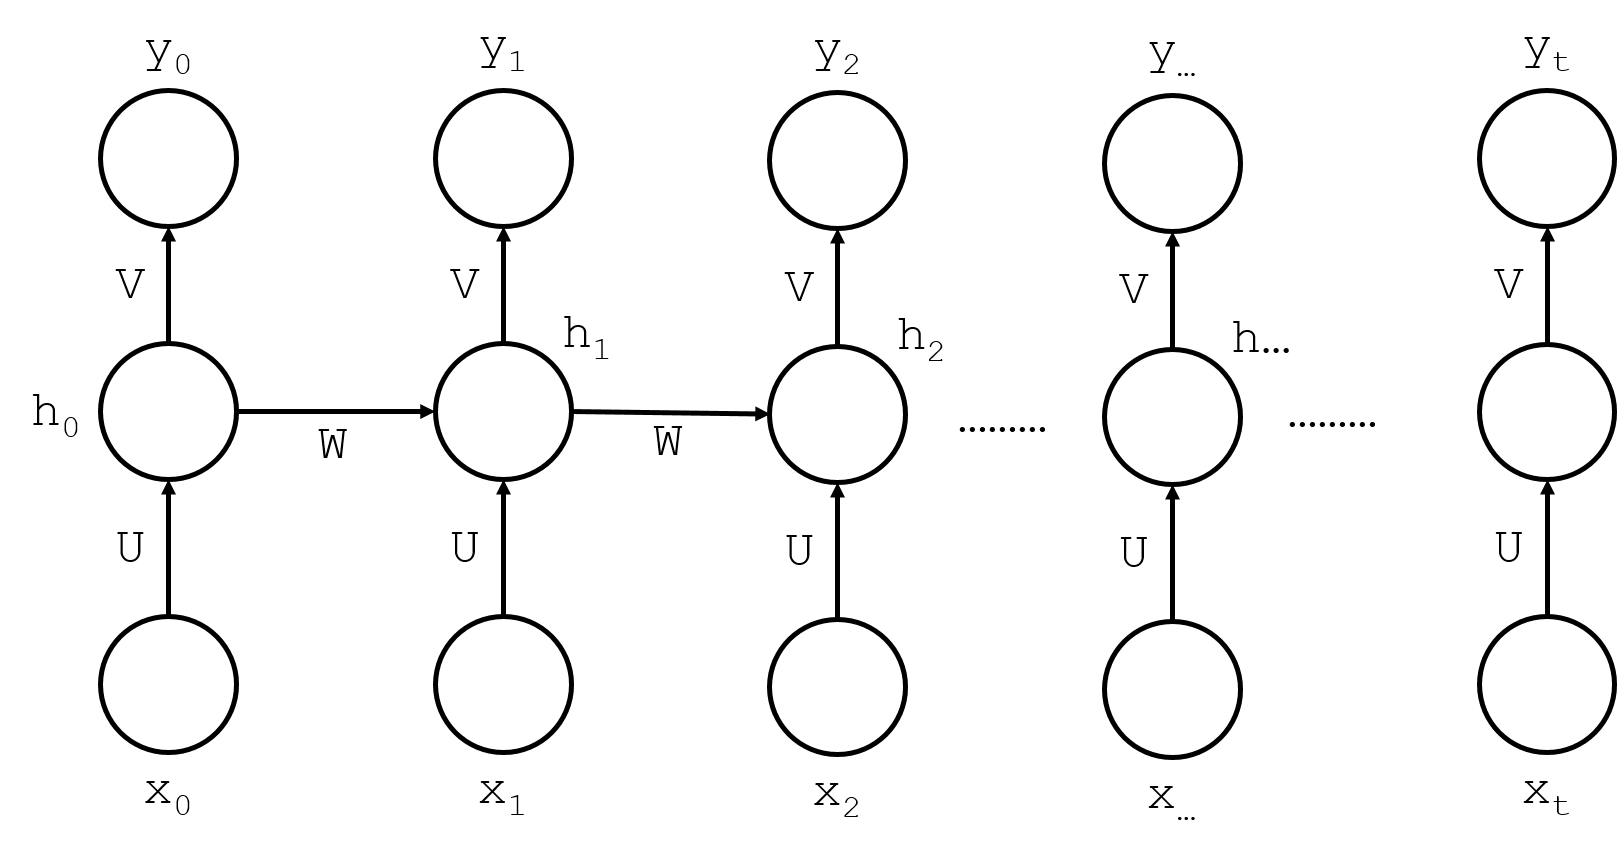
\includegraphics[width=0.55\linewidth]{images/simple_rnn}
	\caption{\textit{Simple Recurrent Neural Network}} {Sumber gambar: \cite{mikolov2010recurrent}}
	\label{fig:simplernn}
\end{figure}

Sebuah jaringan pada RNNs memiliki \textit{input layer} $ x $, \textit{hidden layer} $ s $ dan \textit{output layer} $ y $. Untuk suatu waktu $ t $, \textit{input} RNNs dinotasikan sebagai $ x(t) $, \textit{state} dinotasikan sebagai $ s(t) $ dan \textit{output} dinotasikan sebagai $ y(t) $.

RNNs have demonstrated great success
in sequence labeling and prediction tasks such as handwriting
recognition and language modeling. In acoustic modeling
for speech recognition, however, where deep neural networks
(DNNs) are the established state-of-the-art, recently RNNs have
received little attention beyond small scale phone recognition
tasks, notable exceptions being the work of Robinson [1],
Graves [2], and Sak [3].
\subsection{Deep Learning}
\subsection{Vanilla RNNs}
\subsection{Long Short Term Memory}
\subsection{Penerapan RNNs untuk MER}

\section{Word Embedding}
%-----------------------------------------------------------------------------%
% Cerita umum Word Embedding terlepas dari, kenapa bukan %
% Salah satunya adalah word2vc%
% CBOW vs Skip %

Satu \quran~dibagi sama rata ke dalam 30 bagian, yang masing-masing disebut dengan \f{juz}. Dalam \quran~terdapat 114 \f{surat}, di mana setiap surat terdiri dari beberapa \f{ayat}, bervariasi mulai dari 3 ayat sampai 286 ayat. Total seluruh ayat dalam \quran~ada sebanyak 6,236 ayat. Ayat-ayat \quran~tidak seluruhnya unik, karena ada beberapa pasang ayat yang sama dan ada beberapa pasang ayat yang mirip. Hal ini bisa dideteksi menggunakan algoritma yang akan dijelaskan di Bab \ref{lcs}.

%-----------------------------------------------------------------------------%
\section{Pengenalan Suara Otomatis}
%-----------------------------------------------------------------------------%
Pengenalan Suara Otomatis atau yang lebih umum dikenal dengan \f{Automatic Speech Recognition} (ASR) memiliki beberapa definisi dari sumber yang berbeda. Menurut \cite{forsberg2003speech}, ASR adalah proses yang dilakukan komputer untuk menafsirkan ucapan manusia. Definisi lebih teknis diberikan oleh \cite{Jurafsky:2009:SLP:1214993}, yaitu ASR adalah sebuah sistem untuk memetakan sinyal akustik ke dalam untaian kata. Selain definisi-definisi yang telah disebutkan sebelumnya, \cite{chigier1997automatic} menambahkan bahwa ASR merupakan proses komputasi yang bertujuan untuk menangkap sinyal akustik yang merepresentasikan ucapan dan menentukan kata-kata yang diucapkan menggunakan pencocokan pola.

Teknik dalam membangun sistem ASR berbeda-beda, namun secara garis besar ada kesamaan. Sistem pengenalan suara umumnya memiliki sekumpulan model akustik dan bahasa yang direpresentasikan sebagai pola, dan disimpan dalam sebuah basis data komputer. Model-model ini kemudian dibandingkan dengan sinyal yang ditangkap. Untuk sistem ASR yang mengandung sedikit kosakata (kurang dari 50 kata), sebuah model dapat merepresentasikan sebuah kata. Namun untuk kosakata yang lebih dari 50 kata, proses pemodelan dan algoritma pengenalan membutuhkan komputasi yang banyak dan tidak praktis. Oleh karena itu, sistem dengan kosakata yang banyak (lebih dari 1000 kata) membuat sebuah model yang merepresentasikan komponen yang lebih kecil dari kata, sebagai contoh adalah \f{fonem}. Deretan fonem dapat dirangkai untuk menghasilkan sebuah model kata.

\cite{juang2005automatic} dalam artikelnya yang berjudul \f{Automatic Speech Recognition -- A Brief History of the Technology Development} menjelaskan bahwa saat ini teknologi ASR sudah tersedia secara komersial, walaupun hanya mampu menjalankan tugas-tugas yang terbatas. Teknologi ini memungkinkan mesin untuk menanggapi perintah manusia melalui suara dengan baik. Namun teknologi tersebut masih jauh dari kemampuan untuk bercakap-cakap dengan manusia dalam berbagai topik bebas. Perkembangan dalam bidang sains dan teknologi semakin mendorong sistem ASR untuk menjadi sistem yang mampu mengenali dan memahami ucapan manusia dengan baik.

Sejarah singkat mengenai perkembangan ASR dapat dikelompokkan ke dalam beberapa era. Dimulai pada sekitar tahun 1960, di mana pada saat itu telah berhasil dikembangkan teknologi yang mampu mengenali kosakata dalam skala kecil (10 sampai 100 kata). Pengenalan ini dilakukan dengan mengenali kata demi kata secara terpisah berdasarkan sifat-sifat \f{acoustic-phonetic} yang terdapat dalam suara. \f{Acoustic-phonetic} adalah ilmu tentang karakteristik akustik dari suara. Kunci dari keberhasilan teknologi ASR di era ini adalah analisis \f{filter-bank}, metode normalisasi \f{simple time}, dan permulaan dari metodologi \f{dynamic programming} yang canggih. \f{Filter-bank} adalah pembagian sinyal \f{input} $x(n)$ ke dalam himpunan sinyal analisis  $x_1(n), x_2(n), \ldots$, yang masing-masing berkorespondensi terhadap wilayahnya di dalam spektrum $x(n)$.

Sekitar tahun 1970, teknologi yang berkembang mampu untuk mengenali kosakata dalam skala sedang (100 sampai 1000 kata). Kunci perkembangan teknologi di era ini adalah model pengenalan pola (\f{pattern recognition}), permulaan metode \f{Linear Predictive Coding} (LPC) untuk merepresentasikan spektrum, metode \f{pattern clustering} untuk \f{speaker-independent recognizers}, dan permulaan metode \f{dynamic programming} untuk menyelesaikan permasalahan \f{connected word recognition}. Sekitar tahun 1980, teknologi ASR mampu menangani kosakata dalam skala besar (1000 kata atau lebih). Kunci dari keberhasilan di era ini adalah model statistik \f{Hidden Markov Model} (HMM) dan model bahasa \f{stochastic}.

Teknologi semakin maju pada sekitar tahun 1990. Sistem ASR dengan kosakata berskala besar yang lebih canggih dari era sebelumnya telah berhasil dikembangkan pada era ini, dengan adanya \f{continuous speech recognition and understanding}. Adapun keberhasilan teknologi ASR di era ini berkat metode untuk melakukan \f{stochastic language understanding}, pembelajaran statistik dari model akustik dan model bahasa, permulaan \f{finite state transducer framework} (dan juga \f{FSM Library}), serta metode untuk determinasi dan minimalisasi untuk implementasi sistem \f{speech understanding} yang efisien dengan kosakata berskala besar. Akhirnya sekitar tahun 2000, muncul permulaan dari sistem ASR dengan kosakata berskala sangat besar disertai model semantik penuh, terintegrasi dengan sistem sintesis \f{text-to-speech} (TTS), dan \f{multi-modal inputs}.



%-----------------------------------------------------------------------------%
\section{Fitur}
%-----------------------------------------------------------------------------%
Informasi tertentu yang diambil dari data disebut \f{fitur}. Proses pengambilan fitur dari data dinamakan proses \f{ekstraksi fitur}. Dalam sistem ASR, fitur yang populer digunakan antara lain adalah \f{Mel Frequency Cepstral Coefficients} (MFCCs) dan \f{Shifted Delta Cepstral Coefficients} (SDCCs). Implementasi fungsi untuk melakukan ekstraksi fitur MFCCs dan SDCCs akan dijelaskan pada Bab \ref{chap:fungsipendukung}.

	\subsection{Mel Frequency Cepstral Coefficients (MFCCs)} \label{teorimfcc}
	\f{Mel frequency cepstral coefficients} (MFCCs) adalah salah satu fitur modern dalam teknologi \f{speech}, yang diperkenalkan oleh \cite{1163420}. Fitur ini sudah banyak digunakan dalam ASR \citep{young2002htk}, verifikasi \f{speaker} \citep{ganchev2005comparative}, dan juga di dalam identifikasi bahasa lisan \citep{yin2006combining}. MFCCs adalah fitur yang berbasis spektrum \f{short-term}. Dalam penelitian tentang \f{speech}, \f{short term} sering dipilih sebagai fitur dengan asumsi bahwa secara statistik sinyal bersifat stasioner dalam periode waktu singkat. Namun jika terlalu singkat, banyaknya sampel tidak akan cukup untuk menghasilkan estimasi spektrum tepat. Umumnya interval waktu untuk sebuah \fr~adalah 20 ms sampai dengan 40 ms \citep{zahra2013unique}.

  \cite{hitungmfcc} menjelaskan secara garis besar cara menghitung nilai MFCCs dari sebuah data audio. Langkah-langkahnya adalah sebagai berikut.
  \begin{enumerate}
    \item Bagi sebuah sinyal ke dalam beberapa \fr~singkat.
    \item Hitung estimasi \f{periodogram} dari \f{power spectrum} pada setiap \fr.
    \item Terapkan \f{mel filter-bank} ke setiap \f{power spectrum}, lalu jumlahkan energi di setiap \f{filter}.
    \item Hitung nilai logaritma dari seluruh energi \f{filter-bank}.
    \item Hitung nilai \f{discrete cosine transform} (DCT) dari logaritma energi \f{filter-bank}.
  \end{enumerate}



	\subsection{Shifted Delta Cepstral Coefficients (SDCCs)}  \label{teorisdcc}
  \f{Shifted delta cepstral coefficients (SDCCs)} adalah pengembangan dari MFCCs \citep{torres2002approaches}. Untuk menghitung SDCCs diperlukan nilai MFCCs sebagai salah satu parameter dalam komputasi SDCCs. Vektor fitur SDCCs diperoleh dengan cara menumpuk \f{delta cepstral} yang dihitung dari beberapa \fr. Selain nilai MFCCs, fitur SDCCs membutuhkan 4 parameter tambahan sebagai berikut.
  \begin{enumerate}
    \item N: banyaknya koefisien-koefisien \f{cepstral} yang dihitung pada setiap \fr
    \item \f{d}: waktu untuk \f{advance} dan \f{delay} untuk komputasi \f{delta}
    \item \f{P}: pergeseran waktu antarblok berurutan
    \item \f{k}: banyaknya blok di mana koefisien \f{delta} disambungkan untuk membentuk vektor fitur akhir
  \end{enumerate}
  
  Menurut \cite{zahra2013unique}, ide dari perhitungan ini adalah menghitung jarak antara pasangan N koefisien \f{cepstral} paralel yang dipisahkan oleh waktu \f{advance} dan \f{delay} \f{t}, dilakukan pada \f{k} blok dengan waktu geser \f{P} antarblok yang berurutan. Semua nilai jarak ini kemudian disatukan menjadi sebuah vektor. Langkah ini dilakukan secara iteratif dari awal sampai akhir \fr~pada \f{speech}, sehingga diperoleh kumpulan vektor yang menjadi nilai SDCCs. Gambar \ref{fig:hitungsdcc} mengilustrasikan bagaimana cara menghitung sebuah vektor SDCC.
  \begin{figure}
    \centering
    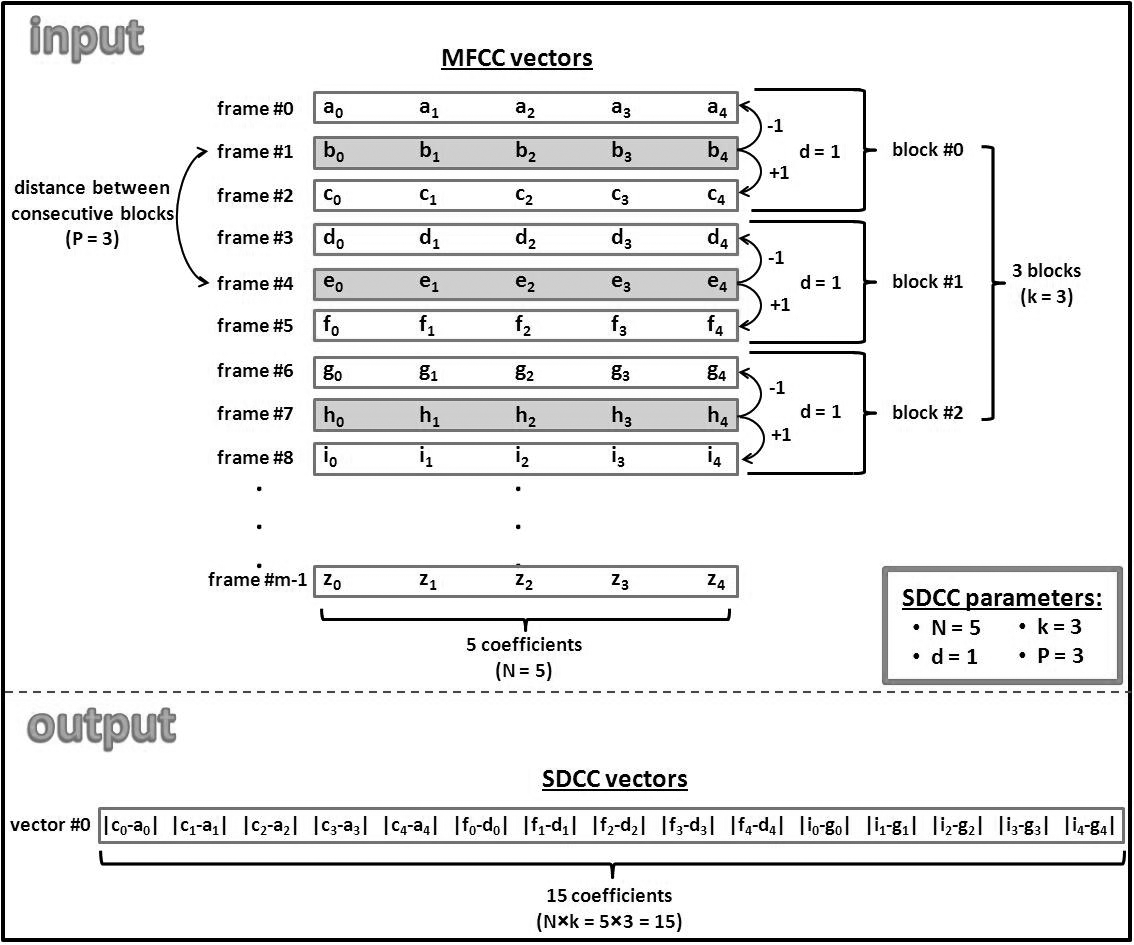
\includegraphics[width=\linewidth]{pics/hitung_sdcc_mono}
    \caption{Contoh Perhitungan Sebuah Vektor SDCC}{Sumber gambar: \cite{zahra2013unique}}
    \label{fig:hitungsdcc}
  \end{figure}



%-----------------------------------------------------------------------------%
\section{Longest Common Subsequence (LCS)}\label{lcs}
%-----------------------------------------------------------------------------%
\cite{Cormen:2009:IAT:1614191} menjelaskan tentang algoritma untuk menyelesaikan permasalahan \f{longest common subsequence} (LCS) dalam bukunya yang berjudul \f{Introduction to Algorithms}. Diberikan sebuah barisan (\f{sequence}) $X=\langle x_1,x_2,...,x_m\rangle$. Barisan $Z=\langle z_1,z_2,...,z_k\rangle$ disebut \textbf{\f{subsequence}} dari $X$ jika terdapat barisan menaik $\langle i_1,i_2,...,i_k\rangle$ berupa indeks dari $X$ sedemikian hingga untuk semua $j=1,2,...,k$, terpenuhi $x_{i_j}=z_j$. Sebagai contoh, $Z=\langle B,C,D,B\rangle$ adalah \f{subsequence} dari $X=\langle A,B,C,B,D,A,B\rangle$ dengan barisan indeks yang berkorespondensi adalah $Z=\langle 2,3,5,7\rangle$.

Diberikan dua buah barisan $X$ dan $Y$. $Z$ disebut \textbf{\f{common subsequence}} dari $X$ dan $Y$ jika Z merupakan \f{subsequence} dari $X$ dan $Y$ sekaligus. Sebagai contoh,  jika $X=\langle A,B,C,B,D,A,B\rangle$, dan $Y=\langle B,D,C,A,B,A\rangle$, barisan $\langle B,C,A\rangle$ adalah \f{common subsequence} dari $X$ dan $Y$ sekaligus. Barisan $\langle B,C,A\rangle$ bukan merupakan \f{common subsequence} terpanjang dari $X$ dan $Y$ karena hanya memiliki panjang 3, sedangkan terdapat barisan $\langle B,C,B,A\rangle$ yang memiliki panjang 4 dan juga merupakan \f{common subsequence} dari $X$ dan $Y$. Karena tidak ada \f{common subsequence} dari $X$ dan $Y$ dengan panjang 5, maka barisan $\langle B,C,B,A\rangle$ merupakan \f{common subsequence} terpanjang atau \textbf{\f{longest common subsequence}} (LCS) dari $X$ dan $Y$.

LCS dapat diselesaikan menggunakan \f{dynamic programming}. Prosedur pada gambar \ref{fig:prosedurlcs} menjelaskan cara untuk menghitung nilai LCS. Prosedur tersebut membutuhkan dua buah barisan sebagai \f{input}, yaitu $X=\langle x_1,x_2,...,x_m\rangle$ dan $Y=\langle y_1,y_2,...,y_n\rangle$, lalu memberikan tabel $b$ dan $c$ sebagai \f{output}. Nilai LCS terdapat pada $c[m,n]$.

\begin{figure}
  \centering
  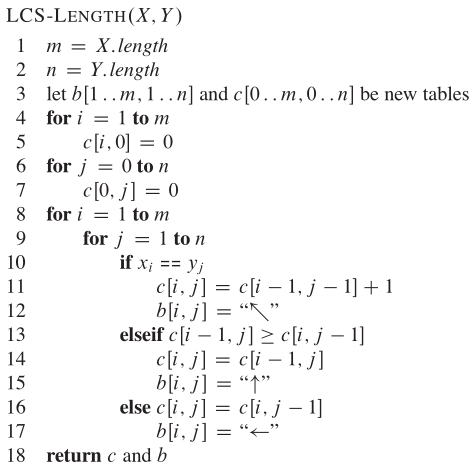
\includegraphics[width=0.7\linewidth]{pics/prosedur_lcs}
  \caption{Prosedur LCS-Length}{Sumber gambar: \cite{Cormen:2009:IAT:1614191}}
  \label{fig:prosedurlcs}
\end{figure}

Gambar \ref{fig:tabellcs} memperlihatkan bagaimana isi tabel yang dihasilkan dari prosedur LCS-Length pada barisan $X=\langle A,B,C,B,D,A,B\rangle$ dan $Y=\langle B,D,C,A,B,A\rangle$.

\begin{figure}
  \centering
  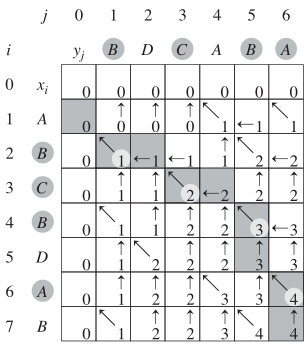
\includegraphics[width=0.55\linewidth]{pics/tabel_lcs}
  \caption{Tabel $c$ dan $b$ yang Dihasilkan oleh Prosedur LCS-Length}{Sumber gambar: \cite{Cormen:2009:IAT:1614191}}
  \label{fig:tabellcs}
\end{figure}


%-----------------------------------------------------------------------------%
\section{Metode \f{Clustering} dan Klasifikasi}
%-----------------------------------------------------------------------------%
Metode \f{clustering} dan klasifikasi adalah dua hal yang mirip. \f{Clustering} mengelompokkan data tanpa diketahui labelnya, sedangkan klasifikasi mengelompokkan data dengan diketahui labelnya.

  %-----------------------------------------------------------------------------%
  \subsection{K-Means Clustering}
  %-----------------------------------------------------------------------------%
  \f{Clustering} adalah proses mengelompokkan data menurut kemiripannya. Ada beberapa metode \f{clustering} yang dikembangkan oleh peneliti, salah satunya adalah \f{k-means clustering}. Metode ini mengelompokkan data menurut kedekatannya ke dalam \f{k} kelompok. Data dalam \f{k-means clustering} berupa sebuah vektor, sehingga kedekatan dua buah vektor ditentukan oleh jarak dari dua buah vektor tersebut. Jarak dua buah vektor salah satunya dihitung menggunakan \f{euclidean distance}. \cite{anton2010elementary} menjelaskan tentang \f{euclidean distance} dalam bukunya yang berjudul \f{Elementary Linear Algebra} sebagai berikut. Jika $\mathbf{u} = (u_1,u_2,...,u_n)$ dan $\mathbf{v} = (v_1,v_2,...,v_n)$ adalah dua buah titik di dalam $\mathbb{R}^n$, maka \f{euclidean distance} antara $\mathbf{u}$ dan $\mathbf{v}$ didefinisikan sebagai
  \begin{equation} \label{equ:euclideandistance}
    d(\mathbf{u},\mathbf{v})=||\mathbf{u}-\mathbf{v}||=\sqrt{(u_1-v_1)^2+(u_2-v_2)^2+\dots+(u_n-v_n)^2}.
  \end{equation}
  
  \cite{kanungo2002efficient} menjelaskan cara kerja \f{k-means} sebagai berikut. Diberikan himpunan $n$ titik dalam dimensi $d$, $\mathbb{R}^d$, dan sebuah bilangan bulat $K$. Tugas dari \f{k-means} adalah menentukan himpunan $K$ titik dalam $\mathbb{R}^d$, yang disebut \f{centers}, untuk meminimalkan nilai \f{mean squared distance} dari setiap titik ke \f{center} terdekat. \f{Center} dalam istilah lain disebut \f{centroid}. Secara matematis, untuk himpunan \f{disjoint} $S_j$ yang berisi $N_j$ titik, \f{k-means} bekerja dengan cara meminimalkan nilai $J$ pada persamaan
  \begin{equation}
    J = \sum_{j=1}^{K}{\sum_{n\in S_j}{|x_n-\mu_j|^2}},
  \end{equation}
  di mana $x_n$ adalah vektor yang merepresentasikan titik ke-$n$ dan $\mu_j$ merepresentasikan \f{centroid} dari titik-titik dalam himpunan $S_j$ \citep{kmeans}. Walaupun algoritma \f{k-means clustering} tidak menghasilkan solusi \f{global optimum} untuk $J$, namun algoritma ini sering digunakan oleh banyak praktisi karena mudah untuk diimplementasikan.

  Metode \f{k-means clustering} secara singkat terdiri dari langkah-langkah sebagai berikut.
  \begin{enumerate}
    \item Masukkan seluruh titik ke dalam $K$ himpunan secara acak.
    \item \label{hitung_centroid} Hitung \f{centroid} pada setiap himpunan.
    \item \label{kelompokkan} Kelompokkan ulang setiap titik ke kelompok yang memiliki \f{centroid} terdekat dengan titik tersebut.
    \item Ulangi langkah \ref{hitung_centroid} sampai \ref{kelompokkan} hingga syarat berhenti terpenuhi, misalnya tidak adanya perubahan kelompok pada setiap titik.
  \end{enumerate}



  \subsection{Support Vector Machine (SVM)}
  \f{Support Vector Machine} (SVM) adalah metode pembelajaran mesin yang relatif baru untuk klasifikasi biner, yaitu klasifikasi yang hanya terdiri dari dua kelas \citep{svm}. Ide dasar dari SVM adalah mencari \f{hyperplane} yang memisahkan data $d$-dimensi secara linier menjadi dua kelas. Namun data sampel terkadang tidak dapat dipisahkan secara linier, sehingga SVM memperkenalkan konsep \f{kernel induced feature space}, yaitu memetakan data ke dimensi ruang yang lebih tinggi supaya data dapat dipisahkan secara linier. Gambar \ref{fig:svm2d} mengilustrasikan data dalam dimensi 2 yang tidak dapat dipisahkan secara linier. Gambar \ref{fig:svm3d} mengilustrasikan data tersebut setelah dipetakan ke dimensi 3 dengan fungsi $\phi(x,y)=(x,y,x^2+y^2)$, sehingga dapat dipisahkan secara linier menggunakan \f{hyperplane}.

  \begin{figure}
    \centering
    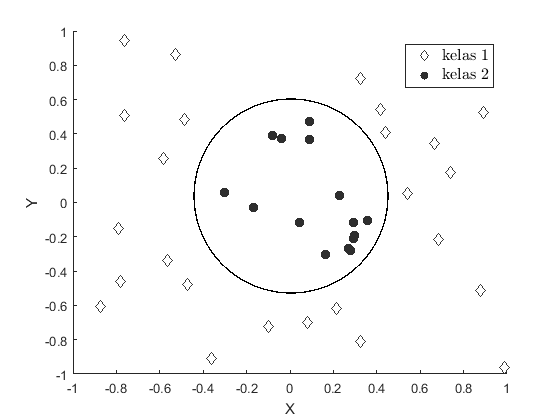
\includegraphics[width=\linewidth]{pics/svm_2db_mono}
    \caption{Ilustrasi Data dalam Dimensi 2}
    \label{fig:svm2d}
  \end{figure}

  \begin{figure}
    \centering
    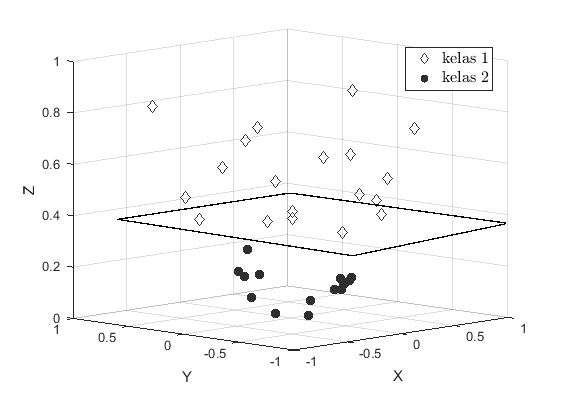
\includegraphics[width=\linewidth]{pics/svm_3db_mono}
    \caption{Ilustrasi Data dalam Dimensi 3}
    \label{fig:svm3d}
  \end{figure}

  Secara matematis, cara kerja SVM dalam melakukan klasifikasi adalah sebagai berikut. Diberikan $l$ sampel \f{training}, $\{\vec x_i,y_i\}$ untuk $i=1,2,\dots,l$; $\vec x_i\in\mathbb{R}^d$; dan $y_i\in\{-1,1\}$. Semua \f{hyperplane} di $\mathbb{R}^d$ memiliki parameter berupa sebuah vektor $\vec w$ dan sebuah konstanta $b$, yang dinyatakan dalam bentuk persamaan
  \begin{equation}
    \vec w\cdot\vec x+b=0.
  \end{equation}
  Diberikan sebuah \f{hyperplane} $(\vec w,b)$ yang memisahkan data, maka terdapat fungsi
  \begin{equation}
    f(\vec x) = sign(\vec w\cdot\vec x+b)
  \end{equation}
  yang mengklasifikasi data \f{training} dengan benar. Syarat data terklasifikasi dengan benar adalah $\forall_i(f(\vec x_i)y_i \geq 1)$.

  Pemetaan ke dimensi ruang yang lebih tinggi membutuhkan proses komputasi yang lebih banyak, serta dapat membuat proses klasifikasi mengalami \f{overfitting}. Karena itu pemetaan vektor tidak dilakukan dalam SVM secara langsung. Pemetaan terjadi secara tidak langsung di dalam \f{kernel function}. \f{Kernel function} adalah fungsi yang digunakan untuk menghitung nilai perkalian dua buah vektor dalam SVM. \f{Kernel function} $K(\vec{x_a},\vec{x_b})$ menerima \f{input} berupa dua buah vektor dan memberikan \f{output} berupa sebuah nilai skalar. Salah satu contoh \f{kernel function} adalah $K(\vec{x_a},\vec{x_b}) = (\vec{x_a}\cdot\vec{x_b}+1)^2$.



  \subsection{Gaussian Mixture Model (GMM)}
  Menurut \cite{6235282}, \f{Gaussian mixture distribution} atau \f{Gaussian mixture model} (GMM) adalah gabungan dari $L$ komponen \f{Gaussian distribution}. Untuk \f{random variable} satu dimensi, $Y$, \f{probability density function (PDF)} dari $Y$ didefinisikan sebagai
  \begin{equation}
    f_Y(y) = \sum_{i=1}^{L}{\omega_i f_{N(\mu_i,\sigma^2_i)}(y)},
  \end{equation}
  di mana $\omega_i$, $\mu_i$, dan $\sigma^2_i$ secara berurutan menyatakan proporsi, rata-rata, dan varian dari komponen ke-i di \f{Gaussian mixture} \citep{4643623}. PDF adalah fungsi pada suatu distribusi \f{random variable} kontinu yang menyatakan probabilitas suatu nilai berada pada interval distribusi tersebut.

  Untuk mempertahankan karakteristik dari \f{probability distribution}, parameter memiliki batasan yaitu, $0<\omega_i\leq1$~dan~$\sum_{i=1}^{L}{\omega_i=1}$. Menurut buku \f{Applied Statistics and Probability for Engineers} yang ditulis oleh \cite{montgomery2013applied}, cara menghitung distribusi dari komponen \f{Gaussian} ke-i, $f_{N(\mu_i,\sigma^2_i)}$, adalah sebagai berikut.
  \begin{equation}
    f_{N(\mu_i,\sigma^2_i)}(x) = \frac{1}{\sqrt{2\pi\sigma^2_i}} e^{(\frac{-(x-\mu_i)^2}{2\sigma^2_i})}.
  \end{equation}

  \cite{5089549} menjelaskan cara menghitung rata-rata ($\mu$) dan varian ($\sigma^2$) dari \f{random variable} $Y$ adalah sebagai berikut.
  \begin{align}
    \mu_Y      &= \sum_{i=1}^{L}{\omega_i\mu_i}\\
    \sigma^2_Y &= \sum_{i=1}^{L}{\omega_i(\sigma^2_i+(\mu_i-\mu_Y)^2)}.
  \end{align}

  Gambar \ref{fig:gmm} menunjukkan \f{probability density} dari \f{random variable} $Y$ yang dimodelkan menggunakan \f{Gaussian distribution} dengan 7 komponen. Jumlah setiap komponen berbobot \f{Gaussian} menghasilkan \f{Gaussian mixture distribution}

  \begin{figure}
    \centering
    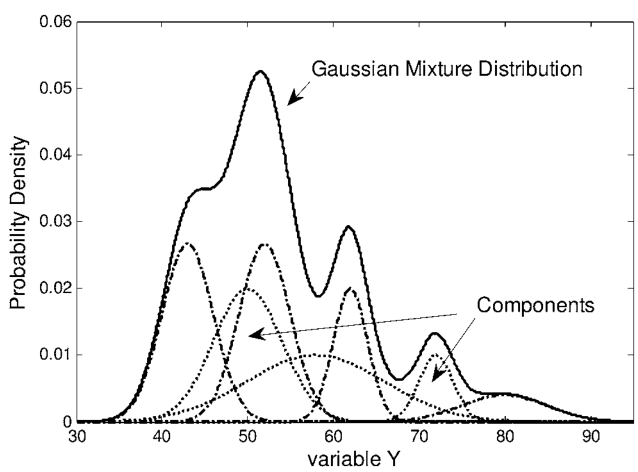
\includegraphics[width=\linewidth]{pics/gmm}
    \caption{\f{Gaussian Mixture Distribution} dengan 7 Komponen}{Sumber gambar: \cite{6235282}}
    \label{fig:gmm}
  \end{figure}

  Keuntungan menggunakan GMM adalah sembarang PDF dengan banyak komponennya terbatas dapat didekati. Biasanya semakin banyak komponen yang ada pada GMM, maka pendekatan tersebut semakin akurat. Metode paling efektif untuk menentukan GMM yang paling mendekati distribusi sampel \f{random variable} $Y$ adalah menggunakan algoritma \f{expectation maximization} \citep{singh2010statistical}.


\section{Evaluasi} \label{chap:evaluasi}
Hasil pada klasifikasi biner dapat dikategorikan menjadi dua, yaitu \f{true} (+) dan \f{false} (-). Perbandingan hasil klasifikasi dengan hasil yang diharapkan dapat dilihat pada tabel \ref{table:kontingensi}.

\begin{table}
  \centering
  \caption{Kontingensi}
  \begin{tabular}{|c|c|c|}
    \hline
    \multirow{2}{7em}{\textbf{Hasil Klasifikasi}} & \multicolumn{2}{c|}{\textbf{Hasil yang Diharapkan}} \\
    \cline{2-3}
    & + & - \\
    \hline
    + & True Positive (TP) & False Positive (FP) \\
    \hline
    - & False Negative (FN) & True Negative (TN) \\
    \hline
  \end{tabular}
  \label{table:kontingensi}
\end{table}

Dari tabel \ref{table:kontingensi} dapat dihitung beberapa metrik evaluasi, yang dapat digunakan untuk melihat dan menganalisis hasil eksperimen. Beberapa contoh metrik evaluasi antara lain sebagai berikut.

\begin{align}
  Accuracy &= \frac{TP+FN}{TP+FN+FP+TN} \label{equ:accuracy} \\
  Precision &= \frac{TP}{TP+FP} \label{equ:precision} \\
  Recall &= \frac{TP}{TP+FN} \label{equ:recall} \\
  F-measure &= \frac{2 \cdot Precision \cdot Recall}{Precision + Recall} \label{equ:fmeasure}
\end{align}

Nilai-nilai pada metrik evaluasi memiliki makna yang berbeda-beda. \f{Accuracy} (persamaan \ref{equ:accuracy}) menyatakan rasio antara banyaknya hasil klasifikasi yang sesuai dengan hasil yang diharapkan dengan seluruh data yang ada. Rasio antara banyaknya hasil positif yang sesuai harapan, terhadap banyaknya hasil klasifikasi yang memberikan nilai positif (+) disebut \f{precision} (persamaan \ref{equ:precision}). Kemudian \f{recall} (persamaan \ref{equ:recall}) menyatakan rasio antara banyaknya yang diklasifikasikan positif dengan banyaknya data yang diharapkan positif. Namun terkadang nilai \f{precision} bersaing dengan nilai \f{recall}. Semakin tinggi nilai \f{precision} umumnya akan membuat nilai \f{recall} semakin rendah, dan sebaliknya. Nilai \f{F-measure} (persamaan \ref{equ:fmeasure}) menyatakan rata-rata harmonik antara nilai \f{precision} dengan nilai \f{recall}.



%-----------------------------------------------------------------------------%
\section{Penelitian Terkait}
%-----------------------------------------------------------------------------%
Penelitian ini membahas sistem \f{automatic speech recognition} (ASR) dalam domain bacaan Al-Qur'an. Beberapa pekerjaan yang sudah dilakukan oleh peneliti sebelumnya terkait bidang ASR dengan domain \quran~antara lain, yang \f{pertama} adalah penelitian yang dilakukan oleh \cite{Muhammad:2010:VCM:1934908.1935467}. Penelitiannya membahas tentang pencocokan suara bacaan Al-Qur'an. Tujuannya adalah membangun sistem yang dapat memberitahukan kesalahan pada pelafalan bacaan \quran~yang tidak sesuai dengan pelafalan yang seharusnya. Penelitiannya menggunakan MFCC sebagai fitur.% Namun tidak dijelaskan secara menyeluruh bagaimana proses pencocokan itu dilakukan dalam penelitiannya. Selain itu, terdapat parameter yang ditentukan sendiri oleh penulisnya tanpa penjelasan, seperti penentuan $threshold\_value = 2,6$ dan $matched \geq 3$. Dalam penelitiannya juga tidak dijelaskan mengenai cakupan data yang digunakan.

Penelitian \f{kedua} dilakukan oleh \cite{putra2012developing} yang dimuat dalam jurnalnya, \f{Developing Speech Recognition System for Quranic Verse Recitation Learning Software}. Jurnal tersebut membahas mengenai pengembangan perangkat lunak untuk membantu pembelajaran dalam membaca Al-Qur'an. Penelitian dalam jurnal tersebut menggunakan MFCC sebagai fitur dan GMM sebagai model.% Walaupun jurnalnya membahas sampai pada tahap pembuatan perangkat lunak, namun penjelasan mengenai ekstraksi fitur dan teknik pemodelannya masih kurang.

Penelitian \f{ketiga} dilakukan oleh \cite{mohammed2015quranic}. Penelitiannya bertujuan untuk mencegah pengubahan suara bacaan \quran~yang banyak tersebar di \f{internet} dan media sosial secara otomatis. Pengubahan yang dimaksud adalah penambahan, pengurangan, atau kesalahan dalam melafalkan bacaan ayat-ayat Al-Qur'an. Penelitian tersebut menggunakan teks sebagai fitur. Proses ekstraksi teks dari audio lebih kompleks dibandingkan dengan proses ekstraksi MFCC. Untuk mengekstrak teks dari suara setidaknya diperlukan model akustik dan model bahasa. Proses ini menggunakan \f{Hidden Markov Model} (HMM) sebagai model untuk mencari tahu teks mana yang paling memungkinkan untuk menjadi \f{output}.% Kekurangan dalam penelitian tersebut adalah laporan penelitiannya hanya mencantumkan hasil yang diharapkan, dan 
Penelitian tersebut memberikan kesimpulan bahwa untuk Bahasa Arab, fitur yang tepat digunakan adalah MFCC dengan model HMM, berdasarkan teknologi yang berkembang saat ini.